\begin{table*}[!t]
    \renewcommand{\arraystretch}{1.3}
	\centering
	\caption{Class Structure Data}
	\begin{tabular}{lrrrrr}
	\toprule
\textbf{Class} & \textbf{Count Class Base} & \textbf{Count Class Coupled} & \textbf{Count Class Derived} & \textbf{Count Line Code} {(Top \% in project)} & \textbf{Count Declared Method} {(Top \% in project)}\\
\midrule
 A & 10 & 272 & 1 & 0.05\% & 0.13\%\\
 B & 3 & 98 & 0 & 0.12\% & 2.2\%\\
 C & 1 & 32 & 0 & 0.7\% & 6.9\%\\
\bottomrule
	\end{tabular}
	\label{fig:ClassStructureAnalysisData}
\end{table*}

\begin{table*}[!t]
    \renewcommand{\arraystretch}{1.3}
	\centering
	\caption{Class Data from Logs For Developer X}
	\begin{tabular}{lrrrrr}
	\toprule
%\textbf{Developer Name} & 
\textbf{Class} & \textbf{\# Sessions} & \textbf{\# Class Visits} & \textbf{\# Other Class Accesses} & \textbf{Time Spent in Class} & \textbf{Time Spent in Other Classes}\\
\midrule
A & 74 & 294 & 78 & 39 hr.\ 34 min.\ 23 sec. & 16 hr.\ 39 min.\ 36 sec.\\
B & 32 & 88 & 52 & 2 hr.\ 54 min.\ 20 sec. & 8 hr.\ 54 min.\ 18 sec.\\
C & 28 & 77 & 52 & 4 hr.\ 28 min.\ 25 sec. & 9 hr.\ 15 min.\ 41 sec.\\
%Developer Y & P & 10 & 45 & 24 & 2 hr.\ 19 min.\ 13 sec. & 1 hr.\ 43 min.\ 12 sec.\\
%Developer Y & Q & 7 & 12 & 20 & 24 min.\ 08 sec. & 2 hr.\ 36 min.\ 32 sec.\\
%Developer Y & R & 5 & 15 & 16 & 53 min.\ 51 sec. & 40 min.\ 18 sec.\\
\bottomrule
	\end{tabular}
	\label{fig:ClassAnalysisData}
	\vspace*{-3mm}
\end{table*}


As previously mentioned, we first establish sessions to investigate developer activity. We define a session as a moving window of time during which a developer is investigating a particular class. For this initial study, we investigated window sizes of 4 hours, 8 hours, 12 hours, and 16 hours.
%\Fix{Will:The picture of sessions replaces these 2 sentences}
%When we define a session of X hours for a class Y we mean to say that starting from the first time the developer visits class Y while navigating we find the last time he visits the same class in X hours. For %each session of class Y that we obtain we study the number of unique classes the developer has visited while in the session as well as the number of times the developer has visited the class Y itself within %the session. 
For each session we calculate the comprehension metrics listed in Section~\ref{sec:DataFramework}. As a change task is completed, the key classes for the task will have large numbers of sessions, as well as large numbers of visits during those sessions. Time spent in the central class and in the other classes during a session helps to assess the effort required to understand the classes visited in the session.
%and the
%\Fix{Will:This next statement "number of such sessions will also be high" confused me because we talked about super blocks and blocks before.  Perhaps starting a new sentence would allow more %explanation.}
%number of such sessions will also be high. 
%We also calculate the time spent by developer in the central class as well as the time spent by the developer spent in other classes in the session of the central class. The time factor gives us an estimation of how well the developer comprehends the class and other classes referenced in the session. We studied such sessions for a moving window of 4 hours, 8 hours, 12 hours and 16 hours. 

\begin{figure}
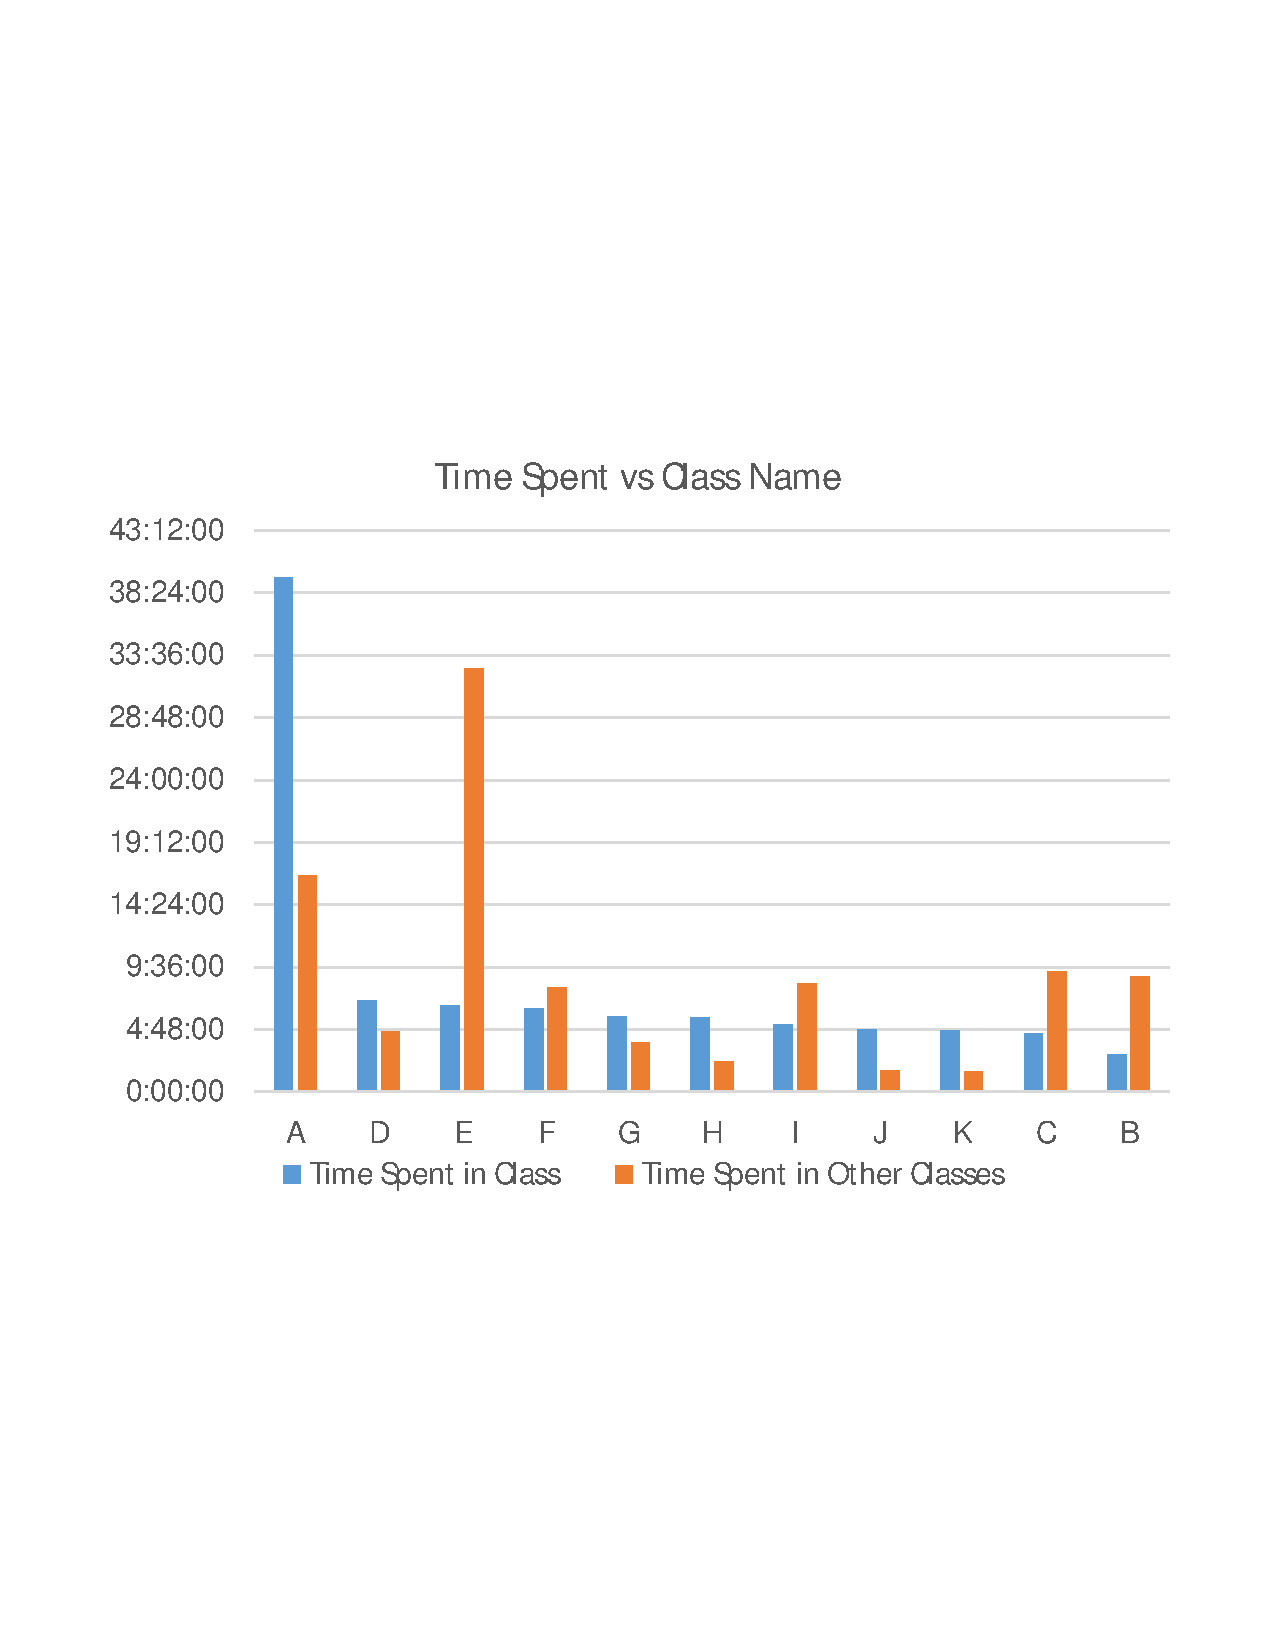
\includegraphics[width=\columnwidth]{ForPaper}
\caption{Time Spent Vs Class Name}
\label{fig:ForPaper}
\vspace*{-6mm}
\end{figure}

The $Blaze$ log for a developer includes all of the navigation activities performed by the developer in the IDE, as well as time-outs for periods of inactivity. We first filtered each developer log, retaining only navigation activities related to classes, time-outs, and IDE exits. Next we calculated the time spent by the developer in each class. We observed that there were instances when the developer visited a class for less than one second before switching to another class. Working on the assumption that the developer could not attain any additional understanding in less than a second,  we attributed such class visits to random clicks and removed all such log entries. We then calculated various parameters to help in identifying the central class, as well the other classes necessary for comprehending the central class.   Finally, we calculated the comprehension metrics defined in Section~\ref{sec:DataFramework}.

%For each sliding window size we calculated the following parameters:
%\begin{itemize}
%	\item[] Number of sessions formed by each class (No Of sessions).
%	\item[] Number of times the class itself has been accessed inside the session (Count No of Class Edits).
%	\item[] Number of unique files visited in each session (Count No of Other Class Accesses).
%	\item[] Time spent in the class that forms the session (Time Spent in Class).
%	\item[] Time spent in all other files in the session (Time Spent in Other Classes). 
%\end{itemize}
We observed that the change in the number of sessions for each class was small when switching between a 4-hour moving window and a 8-hour moving window. The small magnitude of this change indicates that developers do not often work in 8-hour windows, but rather tend to work in 4-hour windows. Moreover, the 8-hour moving window returned the same number of sessions as did the 12-hour and 16-hour windows. Thus, we decided to use the 4-hour sliding window for further analysis.

Table~\ref{fig:ClassStructureAnalysisData} lists the structural code metrics for each of the classes that we have used for this study.  These code metrics were calculated for a project containing 9,888 classes. Class A had the largest $Count~Class~Coupled$ value among all the classes in the project. The other such code metrics for class A were all in the top 2\% when compared to all the classes in the project.
% \Fix{Will:Perhaps express this as percent (like top 1\%} for the project. 
The large values for $Count~Line~Code$ and $Count~Declared~Method$ indicate class A may have the $Large~Class$ smell~\cite{Fowler_etal:1999} and suggest that it perhaps consumes a significant portion of the maintenance effort for the project. 

In our analysis of the code comprehension data, we show the distribution of time for the most active classes in the data set. Figure~\ref{fig:ForPaper} shows a graph of the time spent in class and time spent in other classes for the top 11 classes in the data set. We ordered the data in descending order of time spent in the class. While class A has the greatest time spent in the class and time spent in other classes, the ratio varies among other classes.  In class E  the time spent in other classes while in session is much more than the time spent in the class itself. This shows the fact that there are times when the time spent comprehending other classes is much more than the time spent in the class itself. 

Table~\ref{fig:ClassAnalysisData} lists data for three classes worked on by the developer that we studied. The five rightmost columns list the values for the comprehension metrics that we defined to help quantify \TD. For developer X the number of sessions for class A is large, as are the numbers of (central) class visits and other class visits. This suggests that developer X visited class A often over a long period of time, and also visited other classes frequently while working on class A. The data shows that developer X spent more than 39 hours working on class A and more than 16 hours on other classes during the 74 sessions for class A. The 16 hours that developer X spent during sessions for class A on other classes can be interpreted as the cost of comprehending class A, which can in turn be viewed as \TD.

The second row of the table shows that during the 32 sessions for class B, developer X spent nearly 3 hours on class B but nearly 9 hours on other classes. This indicates that in the sessions for class B, the developer spent three times as long in other classes as he spent in the central class. Considering only time cannot lead to such conclusions, and we need to make sure that the central class for each session is actually central to the task at hand. In the case of class B, there are 32 sessions in which class B was visited 88 times. Thus, we can state that the developer continuously returns to class B, indicating that it is central to the task. 

%Similar patterns can be seen in developer Y where each parameter is indicative of the fact that the considered class is indeed the central class and that the time spent navigating other classes has a significant impact in calculating \TD. 

Considering both the structural code metrics and the comprehension metrics reveals that class A is large and is highly coupled to other classes in the project, and also reveals that the developer spent a large amount of time working on class A. Our preliminary investigation of the code and comprehension metrics revealed several interesting results. When considering the values of $Count~Class~Coupled$, $\#~Other~Class~Accesses$, and $Time~Spent~in~Other~Classes$, we observe that for class A, which is the most highly coupled class in the project, $\#~Other~Class~Accesses$ and $Time~Spent~in~Other~Classes$ are both large. However, for classes B and C, we observe that the values of $\#~Other~Class~Accesses$ and $Time~Spent~in~Other~Classes$ are comparable, even though class C is less coupled than class B. Related to the $Large~Class$ smell, we observe that variation in $\#~Sessions$, $\#~Class~Visits$, and $Time~Spent~in~Class$ aligns with changes in $Count~Line~Code$. Among all three classes, decreases in $Count~Line~Code$ correspond to decreases in the values of $\#~Sessions$ and $\#~Class~Visits$. 

The data presented in this analysis section provides the basic data for calculating interest payments.  There remain parameters to resolve calculation methods for estimation of interest payments and we describe plans to address these in the next section.

%When we look at the parameters that we obtained from the log together with the code metrics we generated for the files we can see how the high numbers of Class A can be seen in both code metrics as well as navigation data. The navigation data shows the time spent by a developer in editing and comprehending class A is on the higher end and the fact that the code metrics shows us that it is the highest coupled class and one of the longest in terms of lines of source code we understand one cause for the high effort spent maintaining Class A.\Fix{Something more needs to be written here but do not know what?}

%Combining the $Time~Spent~in~Class$ and the $Time~Spent~in~Other~Classes$ data for Class A, we estimate the interest payments on that class as 45 minutes per session spent comprehending Class A and related classes.  Against the average comprehension time per session we see this is an increase of x minutes per session meaning that y minutes can be attributed to the technical debt in that class.  If we consider the technical debt in Class B, we calculate 22 minutes per session which against the average of x minutes per session results in y minutes attributable to technical debt.
%
%To compute the interest cost for a given Class, we calculate a portion of the comprehension effort for the first session for that class as principal and consider subsequent sessions as interest payments of further comprehension effort necessary for the class.
